%
% حق نشر 1390-1402 دانش پژوهان ققنوس
% حقوق این اثر محفوظ است.
% 
% استفاده مجدد از متن و یا نتایج این اثر در هر شکل غیر قانونی است مگر اینکه متن حق
% نشر بالا در ابتدای تمامی مستندهای و یا برنامه‌های به دست آمده از این اثر
% بازنویسی شود. این کار باید برای تمامی مستندها، متنهای تبلیغاتی برنامه‌های
% کاربردی و سایر مواردی که از این اثر به دست می‌آید مندرج شده و در قسمت تقدیر از
% صاحب این اثر نام برده شود.
% 
% نام گروه دانش پژوهان ققنوس ممکن است در محصولات دست آمده شده از این اثر درج
% نشود که در این حالت با مطالبی که در بالا اورده شده در تضاد نیست. برای اطلاع
% بیشتر در مورد حق نشر آدرس زیر مراجعه کنید:
% 
% http://dpq.co.ir/licence
%
% در این پرونده چگونگی نوشتن مستندهای سی بیان می‌شود. این استانداردهای بر اساس
% رابطه میان ابزارهای مستند نویسی با Doxygen تعیین خواهد شد.
% مصطفی برمشوری ۱۳۹۰
\chapter{استانداردهای زبان \lr{C/C++}}

در این فصل استانداردهایی برای مستندنویسی کدهایی که به زبان \lr{C/C++} نوشته
می‌شود شرح داده شده است. تمام مواردی که در فصل‌های قبل در مورد مستندنویسی گفته
شد همگی مورد قبول است. در این قسمت نحوه استفاده از این موارد در پروژه‌هایی که به
زبان \lr{C/C++}  نوشته شده‌اند را نشان می‌دهیم. در پروژه‌هایی به این زبان
پرونده‌های سرآیند و پیاده‌سازی وجود دارد که در این قسمت گفته می‌شود که در هر بخش
از پروژه چه مستندهایی نوشته می‌شود.

\section{مستند فنی}
% FIXME : مصطفی ۱۳۹۰-۱۲ :  
% مستند فنی در پرونده‌های سرآیند نوشته می‌شود.
% تمام برچسب‌ها بر اساس استاندار Qt است تا همه را پوشش دهد

در زبان برنامه سازی سی، پرونده‌های سرآیند تنها پرونده‌هایی هستند که بدون ترجمه
انتقال داده می‌شوند. این پرونده‌ها تعیین می‌کند که در پرونده‌های باینری ایجاد
شده چه توابع و موجودیت‌هایی وجود دارد و لینکر چگونه باید پیوندهای مورد نیاز را
ایجاد کند. از آنجا که این پرونده‌ها همواره به عنوان جزئی از خروجی انتقال داده
می‌شوند بهتر است که مستندهای فنی در این پرونده‌ها نوشته شود.

نوشتن مستندهای فنی در پرونده‌های سرآیند منجر به افزایش حجم داده در زمان انتقال
محصول می‌شود. فرض کنید که پروژه‌ای ایجاد شده است، در این صورت در فرآیند انتقال
نیاز است علاوه بر محصول مستندهای تکنیکی نیز به نحوی همراه با محصول انتقال داده
شود، در این صورت مستند فنی علاوه نه تنها به صورت مستقل بلکه همراه با پرونده‌های
سرآیند وجود دارد.

گرچه درنگاه اول افزایش حجم محصول یک ایراد اساسی برای نوشتن مستندهای فنی در
پرونده‌های سرآیند به شمار می‌آید اما با این حال از دیدگاه پیاده ساز به عنوان یک
مزیت در نظر گرفته می‌شود. توسعه دهندگان یک سیستم بدون نیاز به مراجعه به کد
برنامه می‌توانند به مستند فنی آن دست پیدا کنند. بسیاری از محیط‌های مجتمع توسعه
(مانند \lr{Eclipse}) مستندهای نوشته شده در پرونده‌های سرآیند را به عنوان مستند
یک موجودیت برای کاربران نمایش می‌دهد. علاوه بر این می‌توان با استفاده از ابزارهای
مناسب پیش از ایجاد یک محصول، مستندهای فنی موجود در پرونده‌های سرآیند را از محصول
حذف کرد.

\begin{note}
گرچه تنها مستند موجود در پرونده‌های سرآیند، مستند فنی است و توسعه دهندگان سیستم
باید از نوشتن مستند پیاده سازی در این پرونده‌ها خودداری کنند، اما در صورت لزوم
می‌توان برخی از مستندهای پیاده سازی را نیز در پرونده‌های سرآیند نوشت.
\end{note}

زبان برنامه‌سازی \lr{C/C++} یک زبان مترجمی است از این رو بدیهی است که برخلاف
زبانهای قابل حملی مانند \lr{java} قابلیت ترجمه و اجرا برای تمام محیط‌های
نرم‌افزاری و سخت افزاری را نداشته باشد. بدیهی است که در چنین شرایطی مستند فنی
باید به صورت جزئی تمام پیشنیازهای محصول را تعیین کند. برای نمونه فرض کنید که
محصول مورد نظر یک بسته ریاضی است که از دستورالعمل‌های خاصی برای انجام پردازش‌های
خود استفاده می‌کند، در این صورت مستند فنی باید به صورت کامل پردازنده‌های مورد
حمایت را معرفی و نتیجه استفاده از پردازنده‌های دیگر را به صورت کامل تشریح کرده
باشد.

همانگونه که پیش از این نیز اشاره شده، ابزارهای متفاوتی برای ایجاد مستند فنی بر
اساس کد تولید شده در بازار موجود می‌باشد. برای نمونه ابزارهایی مانند \lr{QtDoc}
و \lr{CDoc} دو نمونه از ابزارهایی است که برای ایجاد مستند فنی از پروژه‌هایی که
به زبان برنامه سازی \lr{C/C++} ایجاد شده اند، مورد استفاده قرار می‌گیرند. از این
رو مستند‌های فنی باید به گونه‌ای نوشته شود که بتوان با استفاده از ابزارهای دیگر
نیز مستند فنی مناسبی را ایجاد کرد. برای نمونه در مستندگر \lr{QtDoc} برچسب‌ها را
با استفاده از \textbackslash آغاز می‌شود، از این رو نوشتن تمام برچسب‌ها با استفاده
از این نمادگزاری قابلیت استفاده از این مستندگر را نیز فراهم می‌کند.
علاوه بر این در این مستندگر، برچسب‌های تعریف نشده نادیده گرفته می‌شود از سویی
تمام برچسب‌های تعریف شده در آن، در \lr{Doxygen} نیز تعریف شده است. از این رو
استفاده از تمام برچسب‌های تعریف شده در \lr{Doxygen} برای توسعه مستند فنی بسیار
مناسب است.

مستند فنی هر موجودیت ، در پرونده‌های سرآیند و پیش از آن موجودیت ایجاد می‌شود. در
این مستند باید توضیحات مناسب برای آن موجودیت ایجاد شده و پیوندهای مورد نیاز به
مستندهای وابسته نیز ایجاد شود.

برای نمونه یک کلاس را به عنوان موجودیت در نظر بگیرید، در این صورت علاوه بر
توضیحات کلی در مورد کاربرد و نحوه استفاده از این کلاس، باید اطلاعات دیگری در
مورد نویسنده، تاریخ ایجاد، و نسخه‌هایی که کلاس در آنها ایجاد شده است، به صورت
کامل تشریح شده باشد. برای نمونه کد زیر را در نظر بگیرید:

\begin{latin}
\lstset{language=C++}  
\begin{lstlisting}[frame=single] 
/**
 * \brief <Brief information>
 * 
 * <Detail information>
 * 
 * \see <Other document>
 * \since <First version>
 * \data <Creation Date>
 * \author <Author name>
 */
 class ClassName: public Parent{
 ...
 }
\end{lstlisting}
\end{latin}

همان گونه که در این نمونه مستند قابل مشاهده است، ابتدا به صورت خلاصه در مورد
کلاس نوشته شده و در ادامه به صورت کامل کاربردها و روش‌های استفاده از آن تشریح
شده است. در انتهای مستند اطلاعات جامعی از مستند‌های وابسته، نسخه و
تاریخ ایجاد، و توسعه دهنده آن به صورت کامل آورده شده است. برای نمونه در مستند
زیر تمام اطلاعات مورد نیاز برای یک تابع نوشته شده است:

\begin{latin}
\lstset{language=C++}  
\begin{lstlisting}[frame=single] 
/**
 * \brief <Brief information>
 * 
 * <Detail information>
 * 
 * \see <Other document>
 * \since <First version>
 * \param <param name> <param information>
 * \return <return information>
 */
QString toString(int base, ...);
\end{lstlisting}
\end{latin}

همانگونه که در نمونه بالا قابل مشاهده است ابتدا یک توصیف کوتاه و سپس توصیف کامل
از تابع آورده شده است. در انتهای مستند نیز اطلاعات مورد نیاز در مورد مستندهای
مرتبط، نسخه ایجاد، پارامترهای و خروجی تابع تشریح شده است.

\begin{note}
در پروژه‌هایی که به زبان برنامه نویسی \lr{C} نوشته می‌شود، اطلاعات مشابه در
ابتدایی پرونده سرآیند آورده می شود.
\end{note}

یکی دیگر از موجودیت‌های مهم در پروژه‌های \lr{C/C++} توابع هستند. توابع به عنوان
جعبه‌هایی اجرایی در نظر گرفته می‌شوند که ورودی‌ها را به خروجی تبدیل می‌کنند. در
اینجا نیز علاوه بر توضیحات کلی باید مواردی مانند، پارامترهای ورودی خروجی،
استثناها، نسخه‌ ایجاد شده و مستندهای وابسته نیز در مستند آورده شده باشد.


\section{مستند پیاده‌سازی}
% FIXME : مصطفی ۱۳۹۰-۱۲ : روش نوشتن مستند فنی
% مستند فنی در پرونده‌های cpp نوشته می‌شود و نباید در پرونده‌های سرآیند اورده شود.
% این مستندها ساختار خاصی نداشته و باید از اصول ابتدایی پیروی کنند

مستندات پیاده‌سازی را فقط و فقط باید در پرونده‌های پیاده‌سازی، یعنی پرونده‌های
\lr{.c} یا \lr{.cpp} نوشته شود. هرگز نباید در مورد نحوه پیاده‌سازی یا مواردی از
این دست در پرونده‌های سرآیند مطلبی قرار داده شود.
از آنجا که مستندات پیاده‌سازی برای توسعه‌دهندگانی است که قصد توسعه یا ادامه
پروژه را دارند بهتر است مستندات به گونه‌ای باشد که کار را برای درک کد ساده‌تر
کند. مثلا نیاز نیست برای قسمت‌های ساده مستند نوشت.
معمولا مستندات پیاده‌سازی را باید برای قسمت‌های پیچیده کد نوشت و یا هنگامی که
بخواهیم نکته‌ای را به توسعه‌دهندگان بعدی گوشزد کنیم. بنابراین نباید بی جهت کد را
شلوغ کرد.

پیمان‌نامه\footnote{\lr{Lincense}}  نوعی مستند پیاده‌سازی است یا بهتر بگوییم
مطالبی است که جز مستندات پیاده‌سازی محسوب می‌شود. یک پروژه یا نرم‌افزار ممکن است
پیاده‌سازی‌های مختلفی داشته باشد و هر یک پیمان‌نامه متفاوتی داشته باشد به همین
دلیل باید پیمان‌نامه در مستندات پیاده‌سازی ذکر شود. اگر در یک پیاده‌سازی خاص،
قسمت‌هایی باشند که پیمان‌نامه متفاوتی از دیگر قسمت‌ها دارد باید دقیقا قبل از
قسمت‌ها پیمان‌نامه مربوط به آن آورده شود.

یکی از موارد مهمی که باید در مستندات پیاده‌سازی آورده شود مشخصات سیستمی است.
مستندات سیستمی از جمله مواردی است که هم در مستند فنی می‌آید و هم در مستند
پیاده‌سازی با این تفاوت که در مستند پیاده‌سازی به صورت جزیی‌تر مثلا با ذکر دلیل
نوشته می‌شود. به عنوان مثال فرض کنید تمام یا قسمتی از یک تابع برای سیستم‌عامل
خاصی نوشته شده باشد و یا اینکه تنها روی پردازنده خاصی کار کند آنگاه در مستند
پیاده‌سازی می‌توان ضمن ذکر این موضوع علت آن را هم بیان کرد. مثلا می‌توان در
مستند پیاده‌سازی تابع مورد نظر نوشت: ``این تابع برای پردازنده‌های \lr{Intell}
مدل \lr{Core i7 AVX} به بعد پیاده‌سازی شده است چون در این تابع از مجموعه
دستورالعمل‌های \lr{AVX} استفاده شده است. به همین دلیل این تابع مخصوص
پردازنده‌هایی است که از این مجموعه دستورالعمل‌ها حمایت می‌کنند.''

مستند پیاده‌سازی مکان خاصی برای نوشتن ندارد ولی بهتر است مطالب مربوط به هر قسمت،
موجودیت، قطعه کد و ... قبل از آن بیاید. با استفاده از برچسب‌ها (برچسب‌هایی مثل
\lr{FIXME}، \lr{TODO}، \lr{WARNING} و ...) می‌توان درجه اهمیت مطالب را مشخص کرد.

در یک کار گروه موردی که بسیار به چشم می‌خورد این است که ممکن است بخش‌هایی از
پیاده‌سازی پروژه در مقاطع زمانی مختلف توسط افراد مختلف توسعه، بهبود یا بازنویسی
شود. در این موارد نکته‌ای که باید رعایت کرد این است که مستندات پیاده‌سازی نوشته
شده توسط نویسنده‌های قبلی را نباید حذف کرد. در صورتی که کد ویرایش می‌شود و نیازی
به نوشتن مستند پیاده‌سازی است قبلی مستند جدید به همراه نام نویسنده جدید و تاریخ
ویرایش آن پایین مستند قبلی نوشته شود.
مستندات نویسندگان قبلی در صورتی حذف می‌شوند که قسمت‌های پیاده‌سازی‌ای که آن
مستندات مربوط به آن‌ها هستند به طور کامل از پروژه حذف شوند.



\section{ساختار پروژه}

ساختار کلی پروژه‌های \lr{C/C++} نیز در حالت کلی بر اساس همان ساختاری است که در
گفتار پیش به آن اشاره شده است. اما بر اساس توانایی‌ها و اصول مطرح در زبان این
زبان برنامه سازی مبایست برخی تغییرها را در ساختار کلید لحاظ کرد. در این بخش
تغییرهای مورد نیاز در ساختار کلی پروژه به صورت کلی بررسی خواهد شد.

همانگونه که گفته شده تمام مستندهایی که به صورت مستقیم در رابطه با کد سیستم ایجاد
شده نیست، در یک پوشه جداگانه به نام \lr{doc} ایجاد می‌شود. تمام این مستندها با
پسوند \lr{*.doxy} بوده و حاوی اطلاعات جامعی در مورد مبانی، پیش نیازها، روشهای
نصب و دیگر موارد خواهد بود.

تمام برنامه‌های نوشته شده، مانند پرونده‌های سرآیند و پیاده سازی‌ها در پوشه
\lr{src} قرار می گیرد.
توابع و کلاس‌های تعریف شده در پروژه باید به صورت منطقی (و یا بر اساس فضاهای
تعریف شده در پروژه) در پرونده‌های سرآیند تعریف شده و به صورت مستقیم در مسیر
\lr{src} قرار بگیرد. معادل با هر پرونده سرایند و یا بر اساس منطق سیستم،
پوشه‌هایی ایجاد شده و پیاده سازی تمام توابع و کلاس ها در پرونده‌هایی با پسوند
\lr{*.cpp, *.c, *.cuda}در این پوشه‌ها ایجاد می‌شود.

\begin{figure}
	\centering
    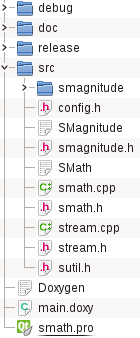
\includegraphics[width=0.25\textwidth]{image/standards-cpp-project-struct}
    \caption[ساختار مورد نیاز برای ایجاد مستند تکنیکی در پروژه‌های \lr{C/C++}]
    {
      
    }
    \label{standards-cpp-struction}
\end{figure}

برنامه‌های زبان برنامه سازی \lr{C/C++} را می‌توان با استفاده از روش‌های متفاوتی
ترجمه کرد. یک روش ترجمه زمانی است که پروژه به صورت کامل تست شده و آماده فاز
تحویل پروژه‌ است. در این فاز با استفاده از برنامه‌های بهینه ساز یک ترجمه بهینه
از پروژه ایجاد می‌شود که به مراتب سریع‌تر از حالت عادی پروژه است. از این رو یک
پوشه به نام  \lr{release} در پروژه ایجاد شده و همواره نتیجه ترجمه نهایی پروژه در
آن ایجاد می‌شود.

ترجمه دیگری که در طی فرآیند توسعه سیستم مورد استفاده قرار می‌گیرد، حالت اشکال
زدا است. در این حالت کدهای اضافه به صورت خودکار به پروزه اضافه شده تا برای دنبال
کردن خط به خط پروژه مناسب باشد. نتایج به دست آمده از این ترجمه نیز در مسیری به
نام \lr{debug} ایجاد می شود.

در نهایت می‌توان با استفاده از ابزارهای مناسب و بر اساس این ساختار، به صورت
خودکار محصول نهایی همراه با مستند تکنیکی را ایحاد کرد. اما پیش از هر چیز نیاز
است که فهرست کاملی از پرونده‌های سرآیند و برنامه‌های نوشته شده ایجاد شود تا
ابزارها بتوانند سرآیندها و برنامه‌های مورد نیاز برای نصب را تعیین کنند. برای
تعیین این پرونده‌ها یک پرونده به نام \lr{<project name>.pro} ایجاد می شود و در
آن فهرست کامل پرونده‌ها ایجاد می‌شود.

\begin{note}
نام این پرونده باید هم نام با پروژه باشد. به یاد داشته باشید که پروژه باید به
صورت کامل در یک پوشه به نام پروژه ایجاد شده باشد، برای نمونه در شکل
\ref{standards-cpp-struction} نه تنها نام پرونده \lr{*.pro} بلکه نام پوشه اصلی
پروژه، هم نام با خود پروژه است.
\end{note}

نام تمام پرونده‌ها با استفاده از کلمه کلید \lr{HEADERS} تعیین می‌شود، در حالت
کلی تعیین پرونده‌های سرآیند به صورت زیر است:

\begin{latin}
\lstset{language=C++}  
\begin{lstlisting}[frame=single] 
HEADERS += <header name> \ 
	... \
	<header name>
\end{lstlisting}
\end{latin}

پرونده‌های پیاده سازی نیز با استفاده از کلمه کلیدی \lr{SOURSES} تعیین می‌شوند.
در حالت کلی این فهرست به صورت زیر ایجاد خواهد شد.

\begin{latin}
\lstset{language=C++}  
\begin{lstlisting}[frame=single] 
SOURCES += <source name> \ 
	... \
	<source name>
\end{lstlisting}
\end{latin}

گاهی ممکن است که پرونده‌های سرآیند و کدهای ایجاد شده تنها برای یک سیستم‌عامل خاص
باشد، در این صورت باید به صورت کامل و تفکیک شده تعیین شوند. در نمونه زیر بر اساس
سکویهای متفاوت کدها و پرونده‌های سرآیند تفکیک شده اند:

\begin{latin}
\lstset{language=C++}  
\begin{lstlisting}[frame=single] 
HEADERS += src/test.h

CONFIG(win) { 
    SOURCES += src/test/win_imp1.cpp \
	src/test/win_imp2.cpp
}
CONFIG(unix) { 
    SOURCES += src/test/unix_imp1.cpp \
	src/test/unix_imp2.cpp
}
\end{lstlisting}
\end{latin}

در این نمونه فرض شده است که برای پرونده سرآیند \lr{test.h} دو نوع پیاده سازی
برای سیستم‌عاملهای یونیکس و ویندوز وجود دارد. از این رو در هر سکو باید
پرونده‌های مناسب ان در محصول نهایی قرار گیرد.
    

\subsection{ساختار پرونده \lr{*.h}}
در یک پرونده سرآیند معمولا تعاریف کلاس‌ها، متدها، توابع و ... آورده می‌شود و
علاوه بر این‌ها باید مستندات این موجودیت‌ها نیز در پرونده‌های سرآیند آورده شود.
ساختاری که برای محل مستندات و تعریف موجودیت‌ها در یک پرونده سرآیند پیشنهاد
می‌شود در قطعه کد \ref{standars-cpp-headers} مشاهده می‌شود.
\begin{latin}
\lstset{language=C++}  
\begin{lstlisting}[frame=single] 
   /*
   *	<License> 
   */
   /**
   *	\file <filenamge>
   *	\date <date>
   *	\brief <a briet documantation about file>
   *	\author <author name>
   *	detailed codumentation about file.
   */
\end{lstlisting}
\label{standars-cpp-headers}
\end{latin}
در ابتدای هر پرونده سرآیند\LTRfootnote{header file} پیمان‌نامه نوشته می‌شود.
نکته اینکه پیمان نامه تنها مستندی است که در مورد پیاده‌سازی است ولی در
سرآیندها هم می‌آید (بنابراین برخلاف سایر مستندات فنی که همگی با \lr{/**}) شروع
می شوند با \lr{/*} شروع می‌شود. پس از پیمان‌نامه مستنداتی در مورد خود پرونده سر‌آیند آورده
می‌شود. مواردی که در این قسمت آورده می‌شود آورده می‌شود عبارتند از:
نام پرونده، تاریخ، نویسنده پرونده،  خلاصه‌ای در مورد پرونده و مستندی در مورد
پرونده به صورت مشروح.

در یک پرونده سرآیند موجودیت‌های مختلفی وجود دارد از جمله تعریف کلاس، متدها و
توابع و غیره. برای تمام این موارد طبق آنچه قبلا گفته شده است باید مستندنویسی
انجام شود. به این ترتیب پس از پیمان‌نامه و مستندات خود پرونده، تعاریف و مستندات
موجودیت‌های مختلف، دیگر محتویات پرونده‌های سرآیند را تشکیل می‌دهند.

\subsection{ساختار پرونده \lr{*.cpp}}
یک پرونده \lr{.cpp} حاوی پیاده‌سازی قسمت‌هایی از پروژه است. مستندات پیاده‌سازی
هر قسمت نیز باید در این پرونده گنجانده شود. همانطور که قبلا هم گفته شد خود
مستندات پیاده‌سازی محل و ساختار خاصی ندارند. اما قالبی برای آن‌ها پیشنهاد می‌شود
که در ادامه شرح داده می‌شود.

 در ابتدای هر پرونده \lr{.cpp} یا \lr{.c} پیمان‌نامه نوشته می‌شود. گاهی ممکن است
 پیمان‌نامه
پرونده‌های سرآیند با پرونده‌هایی که آن سرآیند را پیاده‌سازی می‌کنند متفاوت باشد.
در صورتی که تفاوتی نداشتند می‌توان همان پیمان‌نامه‌ای که در پرونده‌های سرآیند
نوشته می‌شوند را در اینجا نیز قرار داد. مثلا فرض کنید یک گروه نرم‌افزاری یک
مجموعه از سرآیندها را طراحی کرده باشد و پیمان‌نامه خاصی برای آن در نظر گرفته
باشد. سپس گروه‌های دیگری این سرآیندها را پیاده‌سازی کنند. در این مواقع ممکن است
پیمان‌نامه‌ای که گروه‌های پیاده‌ساز به کار می‌برند با پیمان‌نامه گروه طراح
پرونده‌های سرآیند فرق داشته باشد.

پس از پیمان‌نامه مستنداتی در مورد خود پرونده می‌آید. مطالبی از قبیل نام پرونده،
تاریخ، خلاصه‌ای در مورد پرونده و مستندی در مورد پرونده به صورت مشروح (در واقع
همان مواردی که برای پرونده‌های سرآیند نیز مطرح بود). توجه شود که این بخش از
مستند در واقع از نوع مستندات فنی است ولی با این حال در مستندات پرونده‌های حاوی
مستندات پیاده‌سازی آورده می‌شود. سایر مستندات پیاده‌سازی نیز همان مستنداتی است
که برای موجودیت‌های مختلف  پیاده‌سازی شده یا در مورد قطعاتی از برنامه، در
لابه‌لای کدها نوشته می‌شود.

